\catcode"200B=9
\documentclass[zihao=-4]{ctexart}
\usepackage[normalem]{ulem}
\useunder{\uline}{\ul}{}
%********************导言区宏包引入********************
\usepackage{xeCJK}
\usepackage{graphicx}
\usepackage{eso-pic}
% 整页图片命令：用于第一页
\newcommand{\FullPageImage}[1]{%
  \thispagestyle{empty}%
  \AddToShipoutPictureBG*{%
    \AtPageLowerLeft{%
      \includegraphics[width=\paperwidth,height=\paperheight]{#1}%
    }%
  }%
  \null
  \clearpage
}

% 后续页面背景图命令：从调用之后的页面开始生效
\newcommand{\SetPageBackground}[1]{%
  \AddToShipoutPictureBG{%
    \AtPageLowerLeft{%
      \includegraphics[width=\paperwidth,height=\paperheight]{#1}%
    }%
  }%
}
\usepackage{amssymb}
\usepackage{amsmath}
\usepackage{listings}
\usepackage{graphicx}
\usepackage{multicol}
\usepackage{xcolor}
\usepackage{geometry}
\usepackage{fontspec}
\usepackage{setspace}
\usepackage{array}
\usepackage{enumitem}
\usepackage{comment}
\usepackage{tabularx}
\usepackage{longtable}
\usepackage{fancyhdr}
\pagestyle{fancy}
\setlength{\headheight}{15pt}
\usepackage{float}
\usepackage{titlesec}
\usepackage{titletoc}
\usepackage{gbt7714}
\citestyle{gbt7714-numerical}
\usepackage{multirow}
\usepackage{diagbox}
\usepackage{float}
\usepackage{booktabs}
\usepackage{setspace}
\usepackage{caption}
\usepackage{chngcntr}
\usepackage{subcaption}
\usepackage{changepage}
\usepackage{needspace}
\usepackage{pifont}
\usepackage{subcaption}
\usepackage{caption}

%********************Unicode 字符兼容处理********************
\usepackage{newunicodechar}

\newunicodechar{α}{\ensuremath{\alpha}}
\newunicodechar{β}{\ensuremath{\beta}}
\newunicodechar{γ}{\ensuremath{\gamma}}
\newunicodechar{δ}{\ensuremath{\delta}}
\newunicodechar{ε}{\ensuremath{\varepsilon}}
\newunicodechar{η}{\ensuremath{\eta}}
\newunicodechar{θ}{\ensuremath{\theta}}
\newunicodechar{λ}{\ensuremath{\lambda}}
\newunicodechar{μ}{\ensuremath{\mu}}
\newunicodechar{σ}{\ensuremath{\sigma}}
\newunicodechar{ρ}{\ensuremath{\rho}}
\newunicodechar{τ}{\ensuremath{\tau}}
\newunicodechar{φ}{\ensuremath{\varphi}}
\newunicodechar{ϕ}{\ensuremath{\varphi}}
\newunicodechar{ω}{\ensuremath{\omega}}
\newunicodechar{ó}{\'o}
\newunicodechar{í}{\'i}
\newunicodechar{ö}{\"o}
\newunicodechar{́}{}
\newunicodechar{̈}{}
\newunicodechar{Δ}{\ensuremath{\Delta}}
\newunicodechar{Ω}{\ensuremath{\Omega}}
\newunicodechar{×}{\ensuremath{\times}}
\newunicodechar{·}{\ensuremath{\cdot}}
\newunicodechar{√}{\ensuremath{\checkmark}}
\newunicodechar{≤}{\ensuremath{\le}}
\newunicodechar{≥}{\ensuremath{\ge}}
\newunicodechar{→}{\ensuremath{\rightarrow}}
\newunicodechar{、}{\ifmmode\text{、}\else\symbol{"3001}\fi}
%********************Unicode 字符兼容处理********************

\graphicspath{ {include_picture/} }
\let\algorithm\relax
\let\endalgorithm\relax
\usepackage[ruled,vlined]{algorithm2e}
\usepackage{algpseudocode}
\renewcommand{\algorithmicrequire}{Input:}
\renewcommand{\algorithmicensure}{Output:}

\DeclareMathOperator*{\argmax}{arg\,max}
\DeclareMathOperator*{\argmin}{arg\,min}
\DeclareCaptionFont{heixiaosi}{\heiti\fontsize{12pt}{28pt}\selectfont}
\DeclareCaptionLabelFormat{cnfigure}{图#2}
\DeclareCaptionLabelFormat{cntable}{表#2}
\captionsetup[figure]{
  font=heixiaosi,
  labelformat=cnfigure,
  labelsep=space,
  justification=centering,
  singlelinecheck=false
}
\captionsetup[table]{
  font=heixiaosi,
  labelformat=cntable,
  labelsep=space,
  justification=centering,
  singlelinecheck=false
}
\captionsetup[subfigure]{font=heixiaosi, justification=centering}
\counterwithin{figure}{section}
\counterwithin{table}{section}
\renewcommand{\thefigure}{\arabic{section}.\arabic{figure}}
\renewcommand{\thetable}{\arabic{section}.\arabic{table}}
\bibliographystyle{gbt7714-numerical}

%********************导言区宏包引入********************
%********************第三方字体引入********************
\setmainfont[Path=fonts/,
BoldFont = times-new-roman-bold.ttf,
ItalicFont = times-new-roman-italic.ttf,
BoldItalicFont = times-new-roman-bold-italic.ttf
]{times-new-roman.ttf}
\setmonofont[Path=fonts/]{Courier New.ttf}
\setCJKfamilyfont{hwzs}[Path=fonts/]{STKzhongsong.ttf}
\newcommand{\zhongsong}{\CJKfamily{hwzs}}
\setCJKfamilyfont{hwxw}[Path=fonts/]{STKxinwei.ttf}
\newcommand{\xinwei}{\CJKfamily{hwxw}}
%********************第三方字体引入********************

%********************中文字号设置********************
\newcommand{\chuhao}{\fontsize{42pt}{0}}
\newcommand{\xiaochu}{\fontsize{36pt}{0}}
\newcommand{\yihao}{\fontsize{28pt}{0}}
\newcommand{\erhao}{\fontsize{21pt}{0}}
\newcommand{\xiaoer}{\fontsize{18pt}{0}}
\newcommand{\sanhao}{\fontsize{16pt}{0}}
\newcommand{\sihao}{\fontsize{14pt}{0}}
\newcommand{\xiaosi}{\fontsize{12pt}{0}}
\newcommand{\wuhao}{\fontsize{10.5pt}{0}}
\newcommand{\xiaowu}{\fontsize{9pt}{0}}
\newcommand{\liuhao}{\fontsize{8pt}{0}}
\newcommand{\qihao}{\fontsize{5.25pt}{0}}
\newcommand{\bodyfont}{\songti\fontsize{14pt}{28pt}\selectfont}
%********************中文字号设置********************

%********************页边距设置********************
\geometry{
  a4paper,
  left=2.8cm,
  right=2.8cm,
  top=3.5cm,
  bottom=3.5cm,
  headheight=15pt,
  headsep=1.47cm,
  footskip=2.5cm
}
%********************页边距设置********************

%********************段间距设置********************
\newcommand{\setParDis}{\setlength {\parskip} {0pt} }
%********************段间距设置********************

%********************占位图片命令********************
\newcommand{\placeholderimg}[1][0.8\linewidth]{%
  \begin{center}
    \fcolorbox{black}{gray!10}{\parbox{#1}{\vspace{2cm}\centering\textcolor{gray}{\xiaosi [占位图片]}\vspace{2cm}}}
  \end{center}
}
%********************占位图片命令********************

%********************

\begin{document}

%********************第一页整页图片封面********************
\FullPageImage{include_picture/first_page.png}

%********************页眉页脚设置********************
\fancyhf{}
\fancyhead[C]{\songti\fontsize{9pt}{12pt}\selectfont 第十五届“挑战杯”中国大学生创业计划竞赛}
\fancyfoot[C]{\rmfamily\fontsize{12pt}{12pt}\selectfont\thepage}
\setlength{\headwidth}{\textwidth}
%********************页眉页脚设置********************

%********************标题格式设置********************

\setcounter{secnumdepth}{5}
\setcounter{tocdepth}{3}

\renewcommand{\thesection}{\chinese{section}}
\renewcommand{\thesubsection}{\arabic{subsection}}
\renewcommand{\thesubsubsection}{\arabic{subsection}.\arabic{subsubsection}}

\titleformat{\section}[block]
  {\heiti\fontsize{16pt}{28pt}\selectfont}
  {\thesection、}
  {0em}
  {}[]

\titleformat{\subsection}[block]
  {\kaishu\fontsize{16pt}{28pt}\selectfont}
  {\thesubsection.}
  {0.5em}
  {}[]

\titleformat{\subsubsection}[block]
  {\songti\fontsize{14pt}{28pt}\selectfont}
  {\thesubsubsection}
  {0.5em}
  {}[]

\titleformat{\paragraph}[block]
  {\xiaosi\heiti}
  {\theparagraph}
  {0.5em}
  {}[]

\titleformat{\subparagraph}[block]
  {\xiaosi\heiti}
  {\thesubparagraph}
  {0.5em}
  {}[]

\titlespacing{\section}{0pt}{0pt}{0pt}
\titlespacing{\subsection}{0pt}{0pt}{0pt}
\titlespacing{\subsubsection}{0pt}{0pt}{0pt}
\titlespacing{\paragraph}{0pt}{0pt}{0pt}
\titlespacing{\subparagraph}{0pt}{0pt}{0pt}

\titlecontents{section}[0em]{\addvspace{2pt}\filright}
{\contentspush{\thecontentslabel、}}
{}{\titlerule*[8pt]{.}\contentspage}

\titlecontents{subsection}[2em]{\addvspace{2pt}\filright}
{\contentspush{\thecontentslabel.\hspace{0.5em}}}
{}{\titlerule*[8pt]{.}\contentspage}

\titlecontents{subsubsection}[4.5em]{\addvspace{2pt}\filright}
{\contentspush{\thecontentslabel\hspace{0.5em}}}
{}{\titlerule*[8pt]{.}\contentspage}

\titlecontents{section}[0pt]
  {\heiti\fontsize{12pt}{28pt}\selectfont\filright}
  {\contentspush{\thecontentslabel、}}
  {}
  {\titlerule*[8pt]{.}\contentspage}

\titlecontents{subsection}[24pt]
  {\songti\fontsize{12pt}{28pt}\selectfont\filright}
  {\contentspush{\thecontentslabel.\hspace{0.5em}}}
  {}
  {\titlerule*[8pt]{.}\contentspage}

\titlecontents{subsubsection}[48pt]
  {\songti\fontsize{12pt}{28pt}\selectfont\filright}
  {\contentspush{\thecontentslabel\hspace{0.5em}}}
  {}
  {\titlerule*[8pt]{.}\contentspage}

\makeatletter
\renewcommand{\tableofcontents}{%
  \begin{center}
    \heiti\fontsize{18pt}{28pt}\selectfont 目\hspace{1em}录
  \end{center}%
  \vspace{0pt}%
  \begingroup
    \setlength{\parskip}{0pt}%
    \setlength{\parindent}{0pt}%
    \@starttoc{toc}%
  \endgroup
}
\makeatother

\setstretch{1}
\setlength{\parskip}{0pt}
\setlength{\parindent}{2em}
\setlist[itemize]{
  leftmargin=2em,
  topsep=0pt,
  itemsep=0pt,
  parsep=0pt,
  partopsep=0pt
}
\setlength{\intextsep}{28pt}
\setlength{\textfloatsep}{28pt}
\setlength{\floatsep}{28pt}

\renewcommand{\headrulewidth}{0.4pt}

\bodyfont

%********************目录页********************
\newpage
\pagenumbering{roman}
\tableofcontents
\newpage

%********************正文内容********************
\pagenumbering{arabic}

\section{项目概要}

本项目“OmniArm——新一代跨域具身智能机械臂引擎”紧扣“以科技创新推动产业创新、改造提升传统制造业”的赛题要求，面向传统产业自动化设备部署周期长、柔性不足、场景适应能力弱等共性难题，依托我校技术积累与企业场景资源，研发具备快速学习、跨域迁移和自主纠错能力的智能机械臂系统。项目面向消费品、装备、石化化工、冶金和材料等传统优势产业，为复杂作业提供低成本、易部署的智能化解决方案，为传统产业智能化、绿色化、融合化发展提供实践范例。

项目构建“采—训—控”三位一体技术架构，贯通示教数据采集、模型训练与任务执行全过程。在“采”端，自主设计低成本3D打印多模态手持夹爪，集成鱼眼相机和IMU等传感器，使一线人员能够通过自然示教快速采集高质量操作数据；在“训”端，采用基于扩散策略的低样本模仿学习方法，融合视觉与惯性信息，以少量样本完成动作策略学习；在“控”端，集成实时环境感知、动作规划、延迟补偿和闭环纠错技术，使机械臂能够适应物料差异、工位变化和外部干扰，实现“人教即学”、小时级跨场景部署与零样本迁移。

项目客户覆盖消费品制造与生活服务、装备制造、石化化工、冶金材料等领域企业，服务于标准化制作、分拣包装、零部件装配、样品检测、物料转运和危险环境作业等场景。目前，“OmniArm”智能炸制流水线已稳定运行超过1000小时，生产效率达到54篮/小时，验证了系统在真实生产环境中的可靠性与经济性；团队已建立校企联合创新中心，并形成3项专利和1项软件著作权成果。

项目通过定制部署、系统销售、平台授权和数据服务形成多元收入。按照现有财务测算，项目收入预计由2026年的30万元增至2029年的850万元，利润由2万元增至350万元。项目拟融资100万元，其中40\%用于产品迭代与算法研发，25\%用于硬件打样和试点部署，20\%用于市场推广，15\%用于运营及知识产权等支出。

\section{市场分析}

\subsection{选题背景}

东北地区是我国重要的工业基地，在石油化工、冶金材料、消费品制造、食品加工等领域基础雄厚，是维护国家“五大安全”的重要支撑。但东北传统产线普遍存在设备类型多、工艺差异大、自动化系统刚性强等问题。传统机械臂依赖人工编程、示教和固定工位，生产任务变化后通常需要重新标定和调试，难以适应多品种、小批量和柔性化生产。

2023年9月，总书记在新时代推动东北全面振兴座谈会上指出，推动东北全面振兴，关键在科技创新，方向是产业升级。如图\ref{fig:northeast-policy}所示，辽宁和黑龙江省正围绕装备制造、石化化工、食品加工等优势产业推进“智改数转”，建设数字化车间和智能工厂。东北庞大的传统产业存量，既形成了迫切的智能化改造需求，也为智能机器人提供了规模化应用场景。

\begin{figure}[H]
\centering
\begin{subfigure}[b]{0.45\linewidth}
\centering
\includegraphics[width=0.9\linewidth]{黑龙江.png}
\caption{黑龙江}
\end{subfigure}
\hfill
\begin{subfigure}[b]{0.45\linewidth}
\centering
\includegraphics[width=0.9\linewidth]{辽宁.png}
\caption{辽宁}
\end{subfigure}
\caption{东北地区传统产业智能化改造政策}
\label{fig:northeast-policy}
\end{figure}

基于此，“OmniArm——新一代跨域具身智能机械臂引擎”以低成本多模态示教、低样本模仿学习、跨设备迁移和自适应控制为核心，将人工经验快速转化为机械臂作业能力，降低部署、换线和二次开发成本。

\subsection{场景需求}

在传统产业“智改数转”背景下，装备制造、石化化工、冶金材料和食品加工等产业对柔性自动化的需求持续增长。装备制造和汽车零部件生产中的上下料、装配、焊接、打磨及检测等任务换线频繁，而固定程序机械臂重新编程和标定周期较长。

在食品与消费品制造领域，东北拥有丰富的农产品和食品加工基础，但柔性物体、非规则物料以及多规格包装等特点，也对传统自动化提出挑战。分拣、抓取、加工辅助、装盒和码垛等任务需要机械臂根据对象状态实时调整动作。

\begin{figure}[H]
\centering
\begin{subfigure}[b]{0.45\linewidth}
\centering
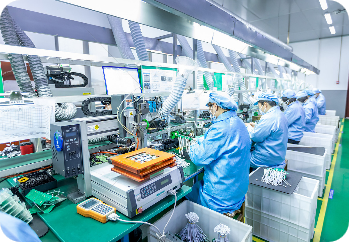
\includegraphics[width=0.9\linewidth]{工厂流水线作业.png}
\caption{工厂流水线作业}
\end{subfigure}
\hfill
\begin{subfigure}[b]{0.45\linewidth}
\centering
\includegraphics[width=0.9\linewidth]{冶金.jpg}
\caption{冶金作业}
\end{subfigure}
\caption{重复任务及高危场景}
\end{figure}

在石化、冶金和材料加工领域，高温、高粉尘及危险介质环境下的物料转运、取样检测和设备维护等任务具有较高安全风险。具备视觉感知、在线纠错和自适应控制能力的机械臂，可减少人员进入危险区域，提高作业连续性与稳定性。

\subsection{痛点分析}

在现代制造业中，机械臂应用主要包括传统工业机械臂和遥操作机器人两类（如图\ref{fig:robot-types}所示）。然而，这两类系统在实际应用中均存在局限，在动态适应性与人机协同效率方面仍有不足，制约了应用范围和生产效率的提升，具体表现为以下技术痛点。

\begin{figure}[H]
\centering
\begin{subfigure}[b]{0.45\linewidth}
\centering
\includegraphics[width=0.9\linewidth]{传统工业机械臂.png}
\caption{传统工业机械臂}
\end{subfigure}
\hfill
\begin{subfigure}[b]{0.45\linewidth}
\centering
\includegraphics[width=0.9\linewidth]{遥操作机器人.png}
\caption{遥操作机器人}
\end{subfigure}
\caption{机械臂应用示意图}
\label{fig:robot-types}
\end{figure}

\subsubsection{传统工业机械臂}

工业机械臂广泛应用于汽车、电子装配等领域\cite{ref1}，但传统方案依赖示教器编程，部署需经过环境规划、网络调试、动作编程、硬件适配和系统测试等环节，人工干预多、周期长、门槛高。同时，其程序固化，难以适应环境和任务变化，跨任务迁移通常需两至三周重新部署调试，难以满足柔性制造和多品种小批量生产需求。

\subsubsection{遥操作机器人}

遥操作机器人通常由远程操作者控制，相比传统机械臂，其在柔性操作与即时反应方面具备一定优势。但当前遥操作系统仍存在自主智能不足的问题，即系统虽具有较高自由度，却缺乏环境感知、任务理解与自主决策能力。

以2025年央视春晚节目《秧BOT》为例，宇树科技的双足机器人虽可完成舞蹈动作，但表演动作需要人工预设并由操作人员控制，缺乏面向环境变化的自主感知与决策机制。同时，遥操作系统自由度高、操作接口复杂，对操作者的专业技能要求较高。在复杂场景下，操作精度较为依赖操作者的经验和实时判断，影响系统的稳定性与可重复性。

综上，传统机械臂和遥操作机器人均难以充分满足现代制造业对高效、灵活和智能化生产的需求。行业亟需开发具备跨域泛化、自主感知和决策能力的新一代机械臂系统以提升生产效率与作业安全水平。

\subsection{相关研究现状}

机器人操作技术主要围绕控制精度、学习效率与场景适应能力发展。早期研究多采用基于模型的轨迹规划方法，Kalakrishnan等人提出通过学习目标函数生成机械臂运动轨迹\cite{ref2}，在结构化场景中具有较高精度，但面对物体位置变化和外部扰动时通常需要重新规划与调试。随后，DAgger等模仿学习方法通过迭代收集专家示范改进策略\cite{ref3}；模型预测控制和深度强化学习则分别从在线优化与端到端控制角度提升复杂任务执行能力\cite{ref4,ref5}，但仍面临计算开销、训练成本和真实设备试错风险等问题。近年来，研究重点逐步转向跨场景泛化。仿真平台与域随机化为策略从仿真迁移至现实提供了基础\cite{ref6}，扩散模型也展现出生成多样化动作序列和提升策略鲁棒性的潜力\cite{ref7}。然而，现有方法在陌生工况适应、不同硬件平台兼容和高速动态响应方面仍有提升空间。在数据获取方面，相关研究已从视觉模仿、零样本任务泛化、VR遥操作、众包示教及互联网视频学习等方向开展探索\cite{ref8,ref9,ref10,ref11,ref12,ref13}。其中，遥操作数据动作信息完整，但通常依赖真实机器人及专业设备；野外视频来源广泛，却普遍缺少精确动作标签，并存在人机具身差距和观测差异，限制了策略直接迁移。

基于上述技术缺口，OmniArm围绕低成本多模态示教、低样本模仿学习、跨设备策略迁移和闭环自主纠错开展系统研发，旨在降低机械臂数据采集与部署门槛，提升其在消费品、石化等场景中的适应能力。


\section{产品介绍}

\subsection{产品形态}

如图\ref{fig:system-architecture}，本项目采用“采—训—控”三位一体架构，将人工示教转化为机械臂可执行策略，使数据采集、模型学习与任务执行形成闭环。

\begin{figure}[H]
\centering
\includegraphics[width=0.85\linewidth]{系统全流程架构.png}
\caption{系统全流程架构}
\label{fig:system-architecture}
\end{figure}

\subsubsection{数据采集}

操作人员使用参考UMI\cite{ref14}设计的多模态手持夹爪，以自然操作方式示范目标任务。系统同步采集视觉、位姿和惯性信息，并自动完成校准、时序对齐与SLAM数据预处理，形成包含环境状态和动作轨迹的训练数据。该方式无需使用示教器逐点编程，可降低数据采集门槛并缩短示教时间。

\subsubsection{模型训练}

模型预训练模块以“硬件无关的扩散策略推理模型”为核心，将示教数据与环境地图进行融合，通过逐步去噪的方式迭代逼近最优动作策略。同时，引入强化学习中的价值评估机制，对采样动作进行即时回报评估，并将结果反馈至模型以更新策略。经过多轮“扩散—评估—更新”循环，模型能够逐步学习最优策略分布，在相似环境中生成高质量动作序列。

\subsubsection{任务执行}

执行端将训练策略与在线感知结果结合，根据物体、工位和障碍状态生成动作指令。运行过程中，系统持续接收视觉和力觉反馈，当物体位置变化或受到外部干扰时及时修正轨迹，形成感知、决策、执行和纠错闭环，保证作业的连续性与稳定性。

OmniArm通过简化部署流程、引入扩散策略推理模型与实时在线规划机制，实现了基于模仿学习的具身智能机械臂系统，做到了“人类教一遍，机器就会做”。

\subsection{3D打印多模态数据采集夹爪}

机械臂技能学习依赖于高质量示教数据的获取。在传统示教流程中，数据采集依赖于机械臂的遥操作，然而这一方法存在显著的缺陷：

操作效率低下：操作人员需要通过手柄或示教器摇杆逐帧驱动机械臂完成目标动作，即使是“倒水”这样极为基础的任务，也要耗费约30秒才能完成一次演示。此过程中，操作者需反复切换平移/旋转模式，经团队实测，人机交互效率不足自然示教的10\%。

动态响应迟滞：传统示教采用位置-速度双闭环控制，且因通信和控制系统的固有延迟，无法实现脉冲式驱动或快速起动（如拍球、投掷），严重影响数据采集效率和质量。经团队实测，其末端最大初速度被限制在0.3m/s以内，难以捕捉人类动作的瞬态特征。

针对上述不足，项目采用基于3D打印的多模态手持数据采集夹爪。该夹爪采用低成本柔性材料一体化打印，内置超广角摄像头和IMU，能够同步捕获高分辨率的视觉、深度和惯性数据。操作人员只需用手握持夹爪，即可在任意场景下对目标物体进行示教：无需固定工作台，无需预设动作点，一次自然演示即可生成完整的多模态数据序列。

\subsubsection{硬件设计详情}

夹爪采用GoPro腕带式摄像头、鱼眼镜头和内置IMU，如图\ref{fig:sensors}所示，可同步记录广角图像、加速度与角速度，捕捉快速起停等动作特征。

\begin{figure}[H]
\centering
\begin{subfigure}[t]{0.3\linewidth}
\centering
\includegraphics[height=3.2cm]{腕带式摄像头_GoPro.png}
\caption{腕带式摄像头GoPro}
\end{subfigure}
\hfill
\begin{subfigure}[t]{0.3\linewidth}
\centering
\includegraphics[height=3.2cm]{原始鱼眼图像.png}
\caption{原始鱼眼图像}
\end{subfigure}
\hfill
\begin{subfigure}[t]{0.3\linewidth}
\centering
\includegraphics[height=3.2cm]{微型惯性测量单元陀螺仪.png}
\caption{IMU陀螺仪}
\end{subfigure}
\caption{多模态传感器示意图}
\label{fig:sensors}
\end{figure}

系统保留原始鱼眼图像作为策略输入，在维持中心区域分辨率的同时压缩周边信息，从而记录夹爪动作及更大范围的环境状态。位姿估计采用基于ORB-SLAM3\cite{ref15}的惯性单目SLAM系统，将图像特征跟踪与IMU姿态约束联合优化；当快速运动造成图像模糊或局部区域缺少视觉特征时，惯性信息可辅助系统短时维持位姿跟踪，为投掷、快速起停等动态动作的数据采集提供支持。

\begin{figure}[H]
\centering
\includegraphics[width=0.5\linewidth]{夹爪_3D_打印.png}
\caption{夹爪3D打印}
\end{figure}

夹爪（如图\ref{fig:gripper-detail}所示）经CAD建模后采用3D打印制作，便于根据任务对象快速调整结构并更换部件，单套硬件成本约200元。其柔性手指通过结构形变提供被动顺应性，可贴合不同物体的几何外形，在保持抓握稳定性的同时降低易碎物品受损风险。

\begin{figure}[H]
\centering
\begin{subfigure}[b]{0.45\linewidth}
\centering
\includegraphics[width=0.9\linewidth]{UMI_数据采集夹爪_CAD_建模图.png}
\caption{UMI数据采集夹爪CAD建模图}
\end{subfigure}
\hfill
\begin{subfigure}[b]{0.45\linewidth}
\centering
\includegraphics[width=0.9\linewidth]{实景抓握图.png}
\caption{实景抓握图}
\end{subfigure}
\caption{多模态数据采集夹爪}
\label{fig:gripper-detail}
\end{figure}

\subsubsection{实用评估}

该夹爪便于携带，可由单人完成不同场景下的自然示教与数据采集，如图\ref{fig:data-collection}所示。

\begin{figure}[H]
\centering
\includegraphics[width=0.75\linewidth]{实景数据采集.png}
\caption{实景数据采集}
\label{fig:data-collection}
\end{figure}

经团队实测，与机械臂遥操作相比，手持夹爪的示教效率提升5倍以上，一次“倒水”示教时间由约30秒缩短至5秒以内，并避免远程通信延迟对快速连贯动作的影响。采集的视觉、位姿和惯性数据可为扩散策略模型提供训练样本，支撑后续的低样本学习、策略泛化和在线自适应。

\subsection{低样本模仿学习模型}

在智能机械臂系统中，如何使机械臂具备快速学习和高效决策能力，一直是研究的关键问题。传统强化学习和监督学习方法往往需要大量标注数据和较长训练时间，尤其在实际应用场景中，数据获取困难且样本稀缺，导致模型训练效率较低，难以应对快速变化的工作环境。因此，如何利用有限样本实现机械臂行为的快速模仿和高效决策，成为提升系统自适应能力的核心挑战。

为此，项目提出基于低样本模仿学习的决策模型，通过多模态数据融合与扩散策略去噪优化，在较少样本条件下实现机械臂动作模仿与任务执行。决策过程分为多模态数据处理、扩散策略构建动作序列和闭环自主训练三个步骤。如图\ref{fig:few-shot-model}所示，该模型通过递进式架构形成跨模态感知与决策闭环。

\begin{figure}[H]
\centering
\includegraphics[width=0.8\linewidth]{低样本模仿学习模型原理图.png}
\caption{低样本模仿学习模型原理图}
\label{fig:few-shot-model}
\end{figure}

\subsubsection{第一步：多模态数据采集与处理}

在低样本模仿学习中，数据的多样性和丰富性对模型训练效果至关重要。然而，在工业应用中，尤其是复杂机械臂任务中，获取并标注大量高质量数据通常成本较高。为此，项目设计多模态数据采集方案，采用相机与陀螺仪相结合的方式提供视觉与动态反馈信息，同步采集RGB图像、位姿和IMU惯性数据。
\begin{figure}[H]
\centering
\begin{subfigure}[b]{0.45\linewidth}
\centering
\includegraphics[width=0.9\linewidth]{夹爪末端旋转数据.png}
\caption{夹爪末端旋转数据}
\end{subfigure}
\hfill
\begin{subfigure}[b]{0.45\linewidth}
\centering
\includegraphics[width=0.9\linewidth]{IMU_数据_3D_轨迹图.png}
\caption{IMU数据3D轨迹图}
\end{subfigure}
\caption{IMU数据}
\end{figure}

通过相机与陀螺仪数据融合，系统能够获得较为全面的环境与运动信息，提升对任务场景的理解能力，并为后续模仿学习提供准确输入。该多模态数据采集方案具有较强灵活性，可适应室内、室外及光线较弱等不同工作环境，并保持数据采集的准确性和稳定性。

\subsubsection{第二步：扩散策略模型与动作序列构建}

为降低真实场景中的数据采集与标注成本，项目引入扩散策略（Diffusion Policy）模型\cite{ref16}，将视觉、位姿等多模态信息作为条件，通过迭代去噪生成连续动作序列，在少量示范数据下学习接近人工操作的轨迹。相较于依赖大量标注样本的方法，该策略能够生成多种可行动作，提升机械臂对物体位置、环境和任务变化的泛化与适应能力，为跨场景部署提供策略基础。

\subsubsection{第三步：自主闭环高效训练}

传统模仿学习方法通常需要人工干预，通过手动调整训练过程实现模型优化，不仅效率较低，而且依赖大量人工标注。为克服这一问题，项目设计自主闭环训练机制，使系统能够自主执行任务，并根据执行反馈调整策略，实现任务的自动化学习。

在自主闭环训练中，模型在执行每一个动作时评估当前状态与目标之间的误差，并根据误差调整策略。每次反馈都会指导模型在下一次迭代中进行修正，从而提高任务模仿和执行精度。通过这种闭环机制，系统能够持续优化策略，逐步逼近目标任务的理想执行效果。

\begin{figure}[H]
\centering
\begin{subfigure}[t]{0.45\linewidth}
\centering
\includegraphics[height=4cm]{视频素材输入示例.png}
\caption{视频素材输入示例}
\end{subfigure}
\hfill
\begin{subfigure}[t]{0.45\linewidth}
\centering
\includegraphics[height=4cm]{训练集与验证集训练损失率.png}
\caption{训练集与验证集训练损失率}
\end{subfigure}
\caption{输入及训练效果示例}
\end{figure}

为提高训练效率，项目在数据处理阶段引入数据增广技术。在团队开展的训练实验中，使用20条示范视频，通过数据增广扩展数据集多样性，使系统能够在较短时间内完成训练收敛。实测结果显示，经过约40分钟训练，模型即可实现低样本条件下的快速收敛，并达到预期任务执行效果。

\subsection{复杂任务创新优化}

随着机械臂技术在实际应用中的广泛推广，复杂任务的高效执行已成为智能机械臂领域亟待解决的问题。传统机械臂控制系统往往难以有效应对复杂且多变的任务环境，因此项目提出三项创新优化技术以提升机械臂在复杂任务中的执行能力：自动纠错与高速应变、多场景适配与零样本迁移、高精度延迟补偿。

\subsubsection{自动纠错，高速应变}

在实际应用中，机械臂执行的复杂任务往往会受到外部干扰或环境变化影响，导致执行不准确或任务失败。例如，在食品处理、装配线操作等任务中，物体位移、碰撞或环境变化均可能干扰机械臂操作，影响任务执行效率和准确性。

为解决这一问题，项目提出基于视觉的自动纠错机制，将视觉编码器（Vision Transformer，ViT）\cite{ref17}与鱼眼相机结合。ViT的视觉编码原理如图\ref{fig:vit-principle}所示，其通过多头注意力机制处理输入图像；鱼眼相机则提供广角视野，覆盖环境中的物体和动态变化，使机械臂能够识别目标物体并及时调整动作。

\begin{figure}[H]
\centering
\includegraphics[width=0.72\linewidth]{ViT_原理图.png}
\caption{ViT视觉编码原理}
\label{fig:vit-principle}
\end{figure}

当外部干扰或环境变化发生时，系统能够定位关键物体并生成新的动作序列，定位结果如图\ref{fig:key-object-localization}所示。例如，在食材分类任务中，机械臂通过视觉识别食材被拿走的情况，迅速调整任务流程，将被取走的食材重新放回原处，确保任务完成。这一机制使机械臂能够在实时变化的环境中保持任务精确度，减少外部干扰导致的任务失败或效率下降。

\begin{figure}[H]
\centering
\includegraphics[width=0.42\linewidth]{定位关键物体.png}
\caption{关键物体视觉定位结果}
\label{fig:key-object-localization}
\end{figure}

\subsubsection{全场景适配，零样本泛化}

随着机械臂在多场景应用中的广泛使用，如何使机械臂快速适应新的工作环境和任务成为关键挑战。传统机械臂系统通常依赖大量示范数据和特定场景编程完成任务，但现实环境动态多变。对于不确定或未知场景，机械臂往往需要重新进行大量数据采集和任务训练，增加部署成本和时间。

\begin{figure}[H]
\centering
\includegraphics[width=0.75\linewidth]{统一行为克隆框架.png}
\caption{统一行为克隆框架}
\label{fig:behavior-cloning}
\end{figure}

面对这一行业难题，项目采用统一行为克隆框架，使机械臂具备较强的通用性和适应性。通过统一人类示教与机械臂设置，利用宽视域鱼眼镜头对齐观察空间，并使用ArUco标签精确追踪夹爪宽度，使机械臂能够在不同环境中灵活应对，无需为每个新场景进行大规模再训练。

此外，项目采用基于运动学的数据过滤方法，提高机械臂在多变环境下的精确度和稳定性。当机械臂基座位置和运动学状态已知时，由SLAM恢复的绝对末端执行器姿态可用于对演示数据进行运动学和动力学可行性过滤。在过滤后的数据集上训练，可确保策略符合具体机械臂的运动学约束，使其面对陌生环境时无需额外数据样本即可迁移已学习技能。

对于摆放茶杯任务，项目在室外陌生场景进行了迁移实验。经团队实测，机械臂任务迁移成功率达到90\%以上，可在不同场景之间切换并完成任务。

\subsubsection{高精度延迟补偿}

在快速抓取、物体抛掷等高精度任务中，机械臂必须精确同步动作时机。尤其在物体抛掷任务中，释放时机稍有偏差便可能导致任务失败。摄像头、机械臂和工业夹爪等硬件在不同系统中的延迟从个位数到数百毫秒不等，传统控制系统难以实现精确的动作同步。

为解决这一问题，项目提出基于延迟自动补偿的轨迹校准算法。该算法实时测量各硬件延迟，并根据延迟值发送补偿指令。推理时，系统将所有观测与延迟最高的数据流对齐，将RGB相机观测降采样至10—20 Hz，再使用图像捕获时间戳对夹爪和机器人本体感知流进行线性插值，并提前发送命令补偿执行延迟，实现精准的动作同步。

\begin{figure}[H]
\centering
\includegraphics[width=0.75\linewidth]{抛掷任务_丝滑流畅_落点准确.png}
\caption{抛掷任务：丝滑流畅，落点准确}
\end{figure}

在物体抛掷任务中，延迟补偿机制使机械臂能够精确控制物体释放时机。经团队实测，抛掷任务准确率达到98.8\%，全场景延迟控制在20毫秒以内，机械臂可流畅完成任务并将物体抛掷到预定位置。

\section{商业分析}

\subsection{目标客户}

本项目客户包括消费品制造与生活服务、装备制造、石化化工、冶金材料等领域企业。“OmniArm”智能炸制流水线已在餐饮场景完成落地验证，证明系统具备柔性操作、标准化出品和连续稳定运行能力。

消费品制造与生活服务客户包括连锁餐饮、中央厨房、食品加工、饮品烘焙、日化及轻工业包装企业。这类客户普遍面临用工成本高、人员流动大、出品一致性不足和柔性物料处理困难等问题。“OmniArm”可应用于炸制、分拣、抓取、装盒、包装和码垛等环节，通过低成本示教、快速部署和跨场景迁移，将人工经验转化为机械臂稳定作业能力。

装备制造企业重点关注多品种、小批量生产中的上下料、装配、打磨和检测，“OmniArm”可降低编程、标定及换线成本；石化化工企业面临高温高压、易燃易爆和有毒介质等风险，系统可用于物料转运、取样检测及替代人工完成危险区域操作；冶金材料企业在高温、高粉尘和重载环境下存在搬运、去毛刺、样品制备及码垛需求，OmniArm可通过视觉感知、低样本学习和在线纠错提升复杂工况适应能力。

从客户画像看，消费品与生活服务企业的决策者主要关注快速落地、用工替代、出品一致性和投资回报；装备制造企业关注柔性生产、换线效率和系统兼容性；石化化工企业关注安全替代、连续运行和危险环境适应能力；冶金材料企业则关注重载作业、复杂工况适应和稳定执行。项目将根据不同行业需求提供相应的系统配置与部署方案。

\subsection{商业模式}

项目构建“联合研发、企业共创、场景交付、技术授权”相衔接的商业模式。依托我校与享刻智能共建的校企联合创新中心，将高校研发能力、企业场景资源和市场渠道有机结合，面向消费品制造与生活服务、装备制造、石化化工、冶金材料等行业同步开展场景验证与市场合作。项目通过定制部署、系统销售、平台授权和数据服务形成收入，实现技术研发、场景验证、产品交付与持续服务的商业闭环。

\subsubsection{联合创新中心与产学研合作}

联合创新中心下设学生技术研发团队和技术授权对接团队。技术研发团队负责数据采集工具、模仿学习模型、控制系统及跨场景迁移能力的迭代，技术授权对接团队负责需求分析、知识产权保护、工程化适配和项目交付。双方以企业真实需求为牵引，按照“需求定义—方案开发—场景验证—产品优化—成果转化”的流程开展合作，使研发成果能够在真实生产环境中快速验证并持续迭代。

随着产品和业务逐步成熟，团队将依托现有专利、软件著作权和场景数据推进公司化运营，通过技术许可、联合开发和成果转化形成稳定合作关系，使联合创新中心既承担技术研发职能，也成为项目连接产业需求和商业市场的转化平台。

\subsubsection{与企业开展战略合作}

“享刻智能”在泛生活服务场景中具备自动化方案设计、设备集成和商业运营经验，可为项目提供真实应用场景、工程化支持和市场反馈。学生研发团队负责核心算法、数据采集和跨场景迁移技术，合作企业负责场景需求提出、系统集成、试点运营和客户反馈，形成优势互补的企业共创机制。“OmniArm”智能炸制流水线已稳定运行超过1000小时，生产效率达到54篮/小时，为消费品与生活服务场景的产品化和规模化复制提供了验证基础。

在工业市场拓展中，项目将与设备供应商、系统集成商及生产企业开展联合验证，围绕装备制造中的装配检测、石化化工中的取样与危险环境辅助作业、冶金材料领域的物料转运和表面处理等任务开发解决方案，降低项目开拓工业客户时的市场拓展与现场交付成本。

\subsubsection{产品销售、技术授权与定制服务}

针对连锁餐饮、中央厨房、食品加工和轻工业包装等客户，项目将成熟能力封装为模块化系统，通过系统销售和标准化部署降低采购、安装和培训成本；针对装备、石化、冶金和材料企业的专业任务，项目提供场景调研、数据采集、工艺规划、模型训练、硬件适配、部署测试和运维升级等定制化服务。各行业客户根据任务标准化程度选择系统销售、定制部署或平台授权方案。

项目收入由四部分构成：定制部署收取方案开发与现场交付费用，是早期形成现金流的主要方式；系统销售通过交付标准化软硬件产品扩大复制规模；平台授权面向中大型企业和系统集成商提供算法引擎、软件平台及知识产权许可；数据服务则围绕多场景采集、模型训练、性能评估和持续优化提供增值服务。该模式既保留定制项目的场景适应能力，也通过产品和平台授权提升可复制性与持续收入占比。

\subsubsection{长远发展}

项目将持续沉淀餐饮加工与包装、装备装配与检测、石化取样与危险操作、冶金材料搬运与处理等任务数据，在保障客户数据安全的前提下建设可复用数据集和测试交流社区，推动产品标准化、模块化和远程运维能力建设。客户拓展将坚持多行业并行验证与典型场景规模复制，逐步参与多场景示教、模型评测和系统部署等标准建设。

随着产品成熟和客户积累，项目收入结构将由早期定制部署为主，逐步转向系统销售、平台授权和数据服务并重，形成可持续的产品收入、许可收入和服务收入，推动智能机械臂从单点项目交付走向规模化应用。


\section{营销策略}

\subsection{SWOT分析}

项目采用“手持示教—扩散策略—跨场景迁移”技术路径，通过低成本多模态夹爪采集人工示范，并利用扩散策略模型学习复杂动作，从而实现对复杂任务的快速掌握。
该技术的核心优势在于：第一，极高的选择性与精度，能精准学习特定任务，不受其他环境因素干扰；第二，响应速度快、部署成本低，项目自主设计的3D打印夹爪硬件成本不足200元，极大降低了用户门槛；第三，卓越的泛化能力，使其在智能制造、餐饮服务、物流分拣等多个领域具有广阔应用前景。该技术已在我校机器人实验室经团队上千次实验验证，并在与“夸父炸串”的商业合作中落地——“OmniArm”智能流水线已稳定运行超过1000小时，生产效率高达54篮/小时，验证了其在真实场景中的可靠性与商业价值。此外，项目背靠“享刻智能”联合创新中心，团队成员均为相关领域的专业人才，能够及时提供技术支持与售后服务，确保优质的用户体验。

项目仍处于商业化初期，标准化产品与服务体系尚未完善，团队的市场拓展和企业运营经验有待积累；同时，初期部署成本仍需降低，品牌认知度仍需通过产品迭代和市场验证持续提升。

东北传统产业智能化升级为项目提供了政策与市场机遇。《数字辽宁发展规划（2.0版）》《吉林省制造业智能化改造和数字化转型行动方案（2023—2025年）》及《黑龙江省加快推动制造业和中小企业数字化网络化智能化发展若干政策措施》\cite{ref18,ref19,ref20}均支持制造业“智改数转”，与项目面向消费品、装备、石化、冶金材料等行业的应用方向相契合。

项目面临市场竞争、技术快速迭代和客户验证周期较长等挑战。行业企业持续投入，要求团队保持研发与工程化能力；客户对系统稳定性、投资回报和品牌可信度仍需持续验证。

\begin{table}[H]
\centering
\caption{SWOT分析矩阵}
\bodyfont
\newcolumntype{Y}{>{\centering\arraybackslash}X}
\renewcommand{\tabularxcolumn}[1]{m{#1}}
\renewcommand{\arraystretch}{1.3}
\newcommand{\swotquad}[1]{%
  \multicolumn{1}{>{\raggedright\arraybackslash}m{\dimexpr(\textwidth-2.2cm)/2-2\tabcolsep-1.5\arrayrulewidth}|}{#1}}
\begin{tabularx}{\textwidth}{|>{\centering\arraybackslash}m{2.2cm}|Y|Y|}
\hline
 & 优势 (Strengths) & 劣势 (Weaknesses) \\ \hline
内部因素 &
\swotquad{快速示教：小时级跨场景部署\newline
成本可控：夹爪硬件不足200元\newline
场景验证：运行超1000小时} &
\swotquad{产品体系：标准化程度不足\newline
运营经验：市场能力待加强\newline
品牌建设：客户认知待提升} \\ \hline
 & 机遇 (Opportunities) & 威胁 (Threats) \\ \hline
外部因素 &
\swotquad{政策支持：“智改数转”\newline
产业需求：柔性生产持续增长\newline
安全需求：高危作业替代} &
\swotquad{行业竞争：企业持续加大投入\newline
技术迭代：研发需持续推进\newline
市场验证：客户决策周期长} \\ \hline
\end{tabularx}
\end{table}

\subsection{竞品分析}

\subsubsection{竞品选择}

基于功能相似性和市场知名度，项目选择宇树科技Z1机械臂、波士顿动力Stretch和越疆X-Trainer作为竞品分析对象。

\subsubsection{竞品定位}

宇树科技Z1机械臂：可搭载于移动机器人的轻量化、低成本准协作机械臂。

波士顿动力Stretch：面向货箱卸载与搬运任务的自主移动机器人解决方案。

越疆X-Trainer：面向机器人示教数据采集与模仿学习的操作平台。

\subsubsection{竞品对比}

项目从整机重量、有效载荷、定制夹爪支持能力、操控接口难度、客户学习成本和应用迁移时间六个方面对OmniArm与竞品进行比较。


由表\ref{tab:robot_arm_comparison}可见，OmniArm机械臂在定制夹爪、操控接口、学习成本和应用迁移时间方面具有一定优势，适用于多类柔性作业场景。各竞品在载荷能力、整机形态或特定任务方面各有侧重，但在定制化和跨场景迁移方面存在不同程度的限制。

{
    \bodyfont

    % 允许表格从当前页开始，并在空间不足时自动续至下一页
    \renewcommand{\arraystretch}{1.0}
    \setlength{\tabcolsep}{4pt}
    \setlength{\LTleft}{\fill}
    \setlength{\LTright}{\fill}

    \begin{longtable}{
        |>{\centering\arraybackslash}m{2.2cm}
        |>{\centering\arraybackslash}m{2.9cm}
        |>{\centering\arraybackslash}m{2.9cm}
        |>{\centering\arraybackslash}m{2.9cm}
        |>{\centering\arraybackslash}m{2.9cm}|
    }
        \caption{机械臂产品对比}
        \label{tab:robot_arm_comparison} \\
        \hline
        产品对比 &
        OmniArm机械臂 &
        UNITREE Z1机械臂 &
        波士顿动力\newline Stretch &
        越疆\newline X-Trainer \\
        \hline
        \endfirsthead

        \caption[]{机械臂产品对比（续）} \\
        \hline
        产品对比 &
        OmniArm机械臂 &
        UNITREE Z1机械臂 &
        波士顿动力\newline Stretch &
        越疆\newline X-Trainer \\
        \hline
        \endhead

        \endfoot
        \endlastfoot

        整机重量
        & 1.2 kg
        & 4.5 kg
        & 100+ kg
        & 11 kg \\
        \hline

        有效载荷
        & 5 kg
        & 2 kg
        & 20 kg
        & 2 kg \\
        \hline

        定制夹爪
        & 支持定制夹爪，适配各种场景
        & 不支持
        & 不支持
        & 不支持 \\
        \hline

        操控接口
        & 简便，支持多场景智能操控
        & 中等，选择器与预编程
        & 较高，需要预编程
        & 较高，自部署前需训练 \\
        \hline

        客户学习\newline 成本
        & 低，端到端自主适应
        & 高，需要模块编程
        & 高，需要模块编程
        & 高，远程录入采集 \\
        \hline

        应用迁移\newline 时间
        & 快，跨域零样本迁移
        & 慢，需要新编程
        & 局限于协作分拣场景
        & 中等，耗时较长 \\
        \hline
    \end{longtable}
}




\section{项目团队}

\subsection{核心团队}

本项目核心团队由五名成员组成，覆盖项目管理、算法研发、硬件集成、合作对接和品牌营销。项目负责人长期从事具身智能系统设计与软件架构研发，负责技术路线、研发进度和资源统筹；其余成员分别承担行为建模与算法优化、嵌入式与ROS系统集成、产业合作及资源协调、品牌建设与市场传播，能够支撑项目从原型研发到场景落地。

\subsection{组织管理}

团队采用扁平化组织架构，设立项目经理岗位统筹全局，设置四个核心职能岗位：算法开发、硬件开发、合作对接、品牌营销。各岗位负责人直接向项目经理汇报，形成信息流畅、反馈快速的管理机制。依据项目实际进展，团队还可根据任务灵活组建专项小组，确保技术研发、对外合作与市场拓展并行推进。


\subsubsection{组织结构与岗位设置}

团队设项目经理统筹全局，下设算法开发、硬件开发、合作对接和品牌营销四个岗位；根据测试、演示和交付任务灵活组成专项小组。

\subsubsection{人员配置与职责分工}

\begin{itemize}[leftmargin=2em]
  \item 项目经理：负责项目整体进度规划、资源调配、财务统筹及团队协调工作，确保项目方向正确、节奏合理。
  \item 算法开发负责人：承担智能算法设计、模型训练与优化任务，主导感知与决策模块的开发。
  \item 硬件开发负责人：负责机器人系统的搭建、硬件结构设计、控制板通信、传感器集成等底层实现。
  \item 合作对接负责人：主要负责对接合作高校、产业合作伙伴与赛事主办方，拓展资源与协同落地场景。
  \item 品牌营销负责人：负责项目对外展示、品牌设计与新媒体推广，建立项目在行业与公众层面的认知度。
\end{itemize}

\subsubsection{团队运营与治理机制}

团队已建立以目标为导向的工作机制，采用“周例会与阶段评审”管理流程，每周检查项目进度，每月开展阶段性复盘，确保任务对齐、质量达标。后续将引入OKR考核机制，以成果输出为主要评价依据，推动成员明确目标并持续改进。

\begin{figure}[H]
\centering
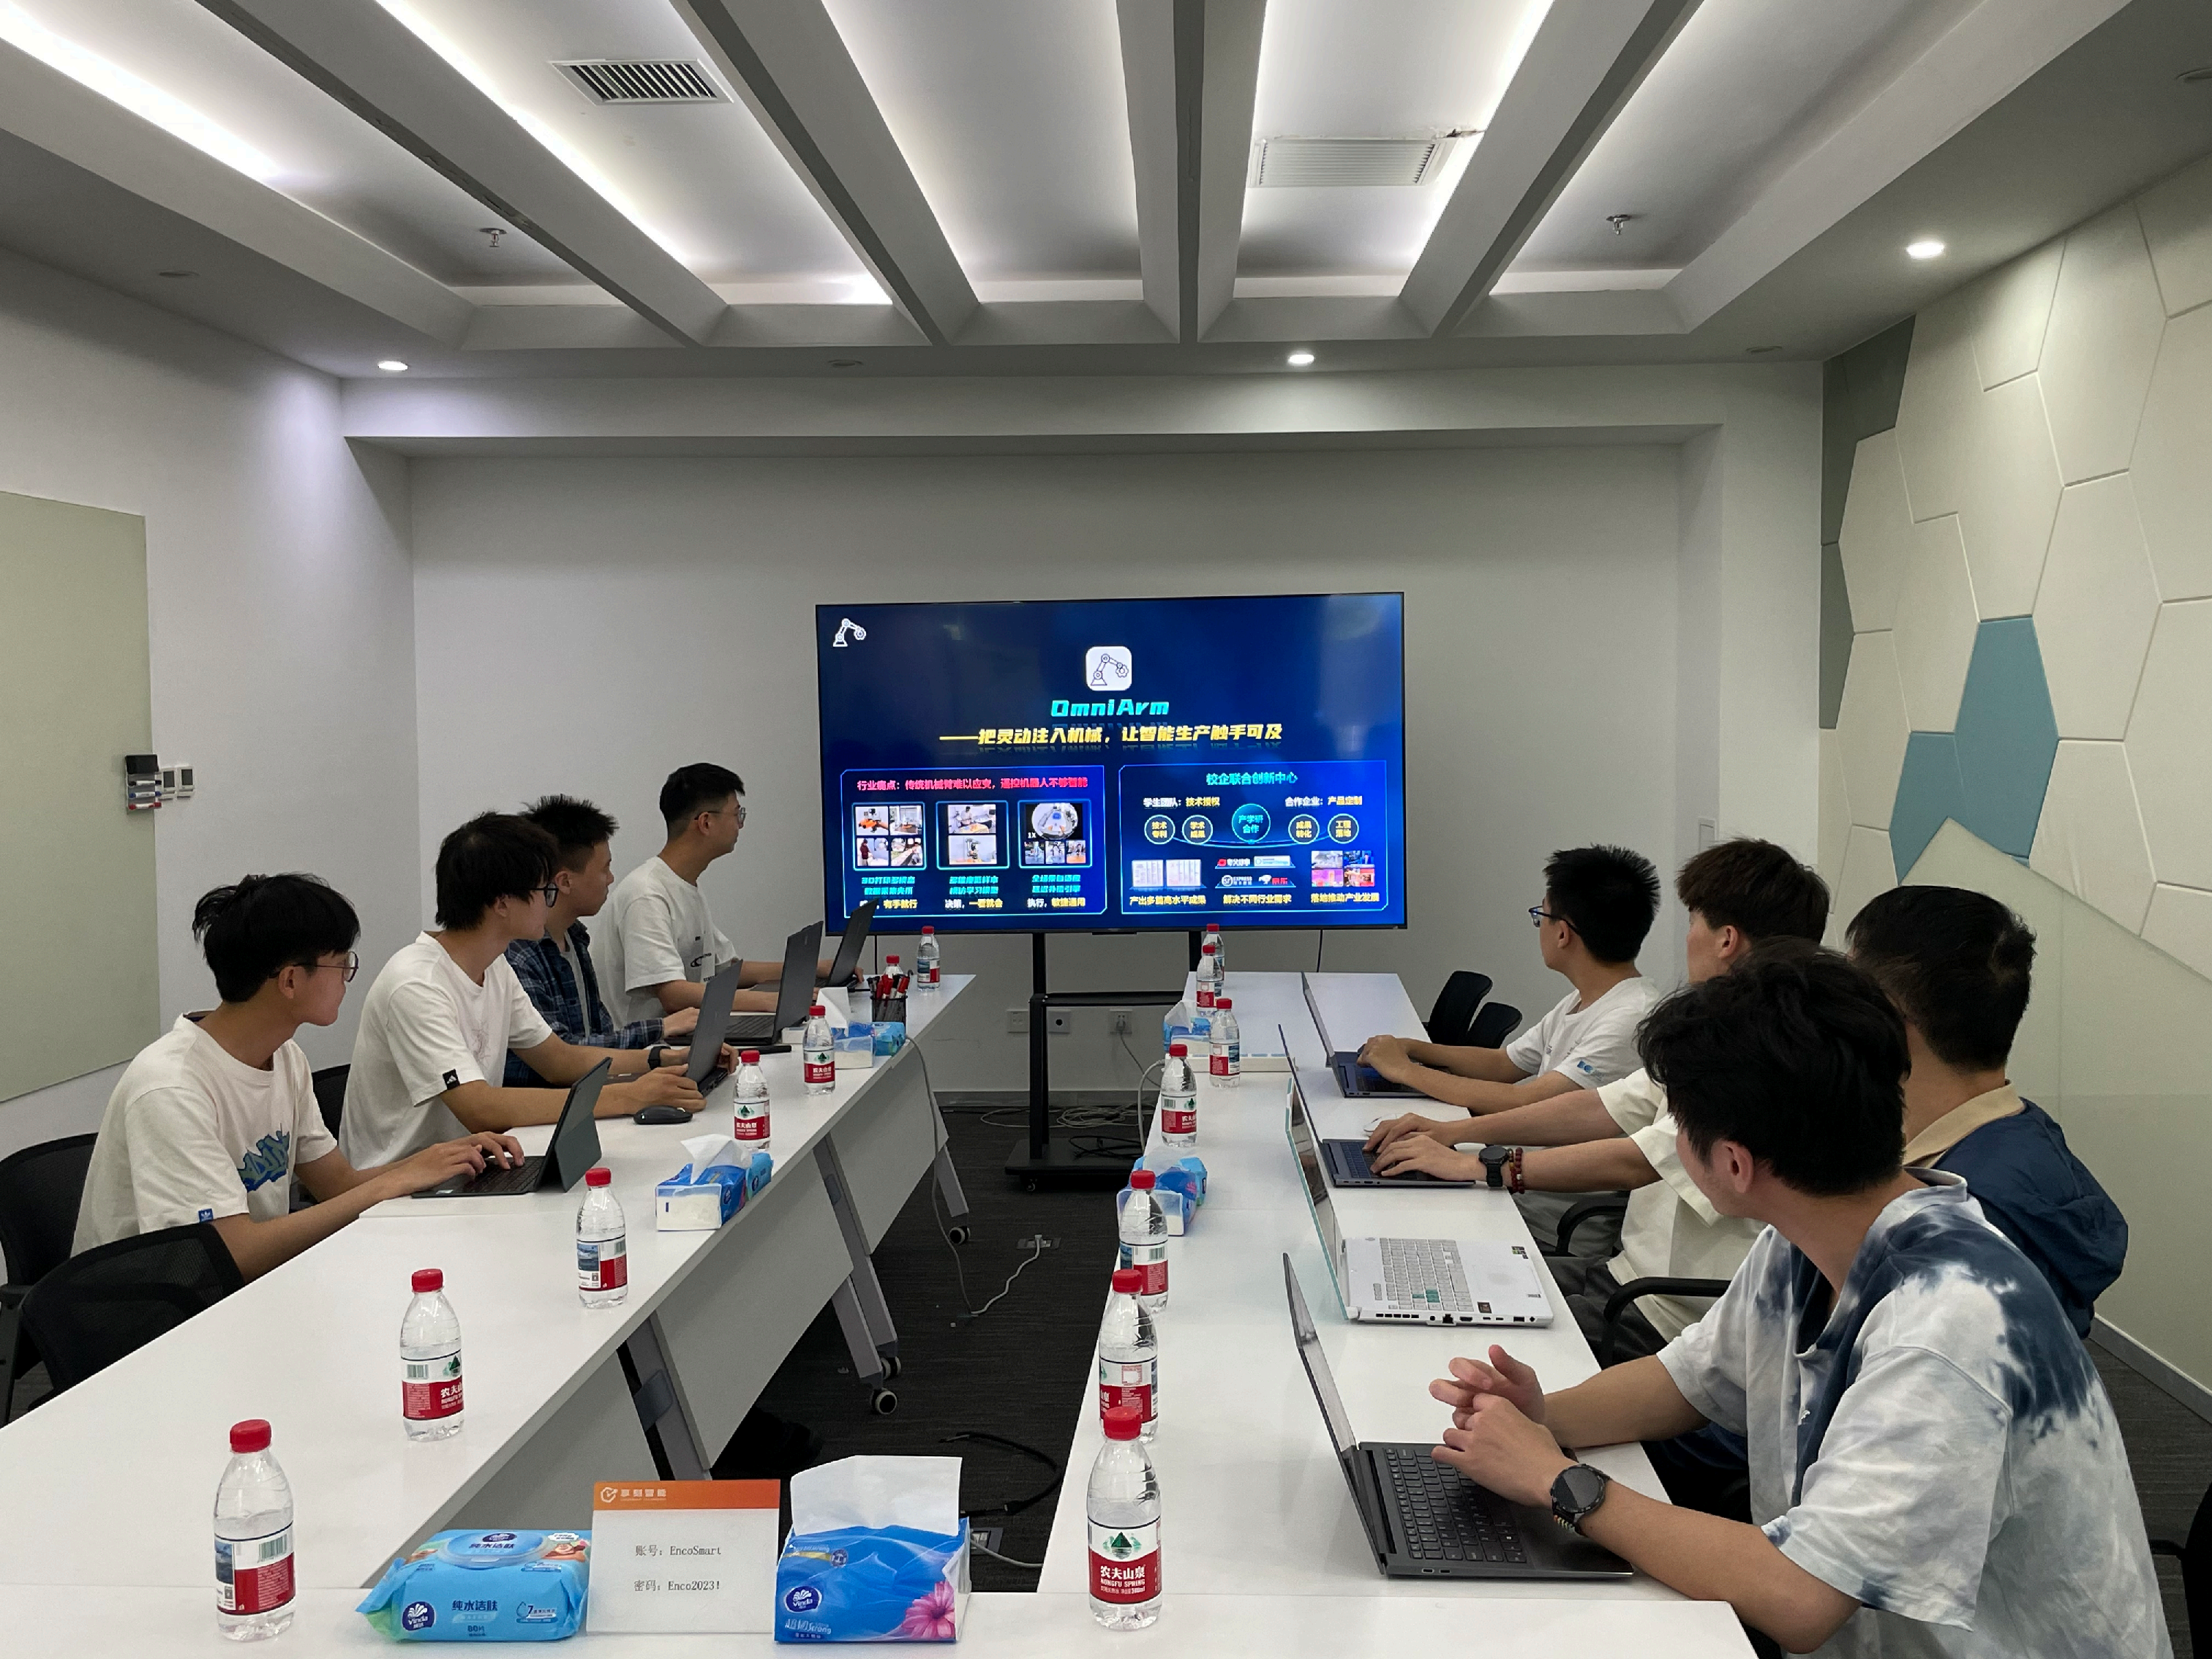
\includegraphics[width=0.65\linewidth]{团队召开每周例会.png}
\caption{团队召开每周例会}
\end{figure}

团队的组织架构兼顾技术研发、市场需求与制度保障，能够支撑项目由技术样机向产品化和商业化稳步推进。

\section{发展规划}

\subsection{项目落地案例}

校企联合研发团队自2024年下半年成立以来，持续推进智能机械臂技术的工程化和场景验证。其中，智能炸制流水线“OmniArm”已在餐饮场景完成落地应用。

2024年9月，项目获得全国首张具身智能食品经营许可证，为相关技术在餐饮场景中的合规应用提供了保障。2025年春节期间，“OmniArm”智能炸制流水线参加海淀新春科技庙会并进行现场展示。团队在展示期间收集了观众对运行效率、稳定性和操作便利性的反馈，为后续产品优化与商业合作提供了参考。


2025年2月，“OmniArm”智能炸制流水线与夸父炸串签署商业合作协议，并在夸父炸串五道口联名店落地运营，标志着项目技术成果开始市场化应用。运营期间，团队围绕生产效率、运营成本和出品一致性开展验证，为后续在其他餐饮门店复制部署积累了经验。


\begin{figure}[H]
\centering
\begin{subfigure}[t]{0.45\linewidth}
\centering
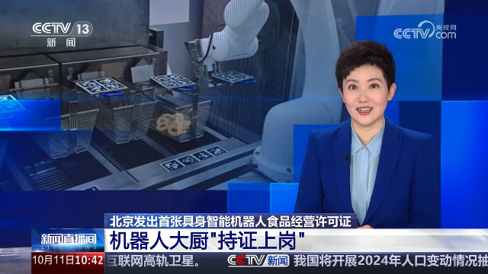
\includegraphics[width=0.9\linewidth]{央视报道_全国首张具身智能食品经营许可证.png}
\caption{央视报道：全国首张具身智能食品经营许可证}
\end{subfigure}
\hfill
\begin{subfigure}[t]{0.45\linewidth}
\centering
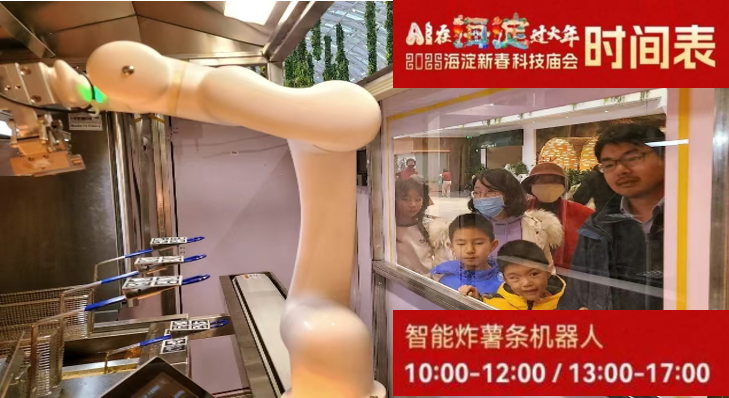
\includegraphics[width=0.9\linewidth]{参展_2025_海淀新春科技庙会.png}
\caption{参展2025海淀新春科技庙会}
\end{subfigure}

\vspace{0.5em}

\begin{subfigure}[t]{0.45\linewidth}
\centering
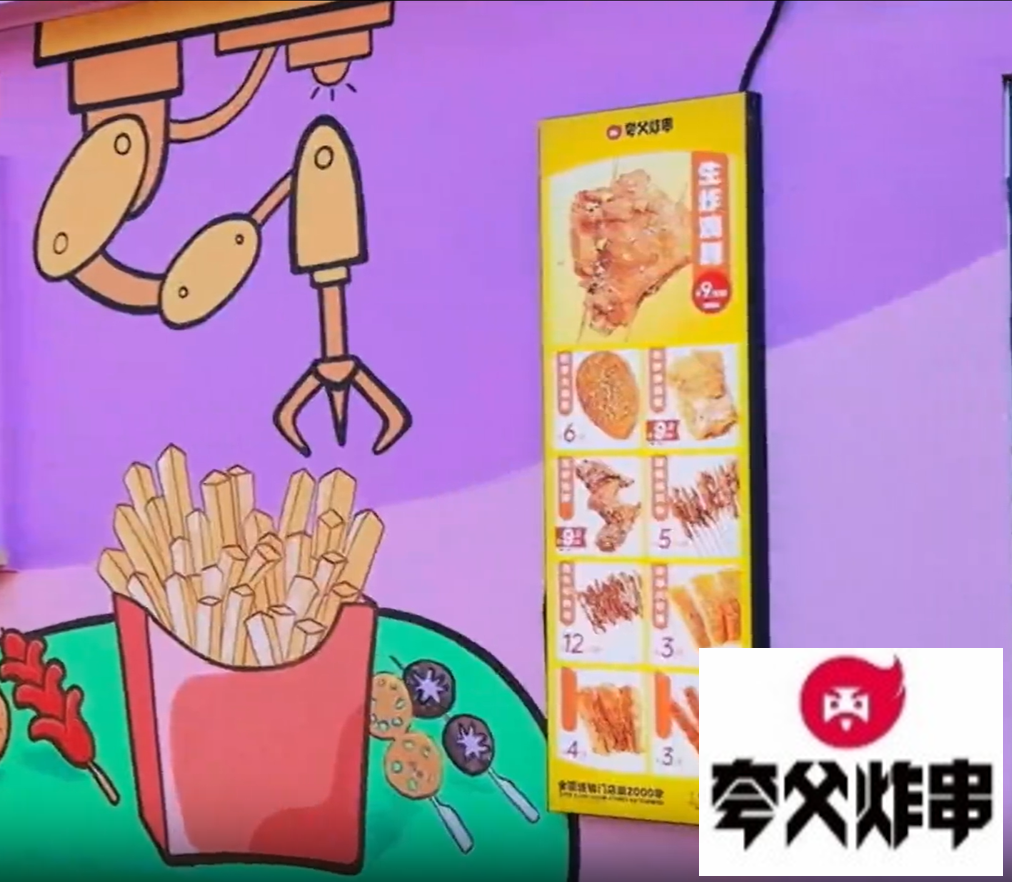
\includegraphics[width=0.9\linewidth]{夸父炸串联名店正式营业.png}
\caption{夸父炸串联名店正式营业}
\end{subfigure}
\hfill
\begin{subfigure}[t]{0.45\linewidth}
\centering
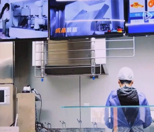
\includegraphics[width=0.9\linewidth]{联名店日常运营.png}
\caption{联名店日常运营}
\end{subfigure}
\caption{落地案例：“OmniArm”智能炸制流水线}
\end{figure}


“OmniArm”智能炸制流水线已稳定运行超过1000小时，生产效率达到54篮/小时。根据项目运营数据，该流水线使相关成本降低25\%以上，验证了系统的连续运行能力和实际应用价值。

上述落地案例表明，“OmniArm”智能炸制流水线已由实验室研发进入实际运营。通过与享刻智能和夸父炸串合作，团队完成了餐饮场景下的工程化验证，为后续向消费品、装备、石化化工和冶金材料等领域拓展提供了实践基础。

\subsection{业务规划}

项目将围绕具身智能机器人系统的研发、落地和生态建设，分五年三阶段推进：

\subsubsection{第一阶段：初创期（2026-2027年）——实现商业闭环，完成首批企业定制与授权合作}

初创阶段，团队将重点开展核心技术研发和产品原型迭代。2025年完成多模态手持示教系统与策略泛化算法的开发和集成，构建软硬件一体化的具身智能示教平台原型，并在校内完成2-3个试验场景部署。

2026年将推进产业化验证，完成不少于5家企业的定制化部署合作，覆盖柔性制造、教育装备和轻工业等领域，实现首批项目营收并初步验证商业模式。同时启动产品标准化与模块化改进，完善团队架构和知识产权布局。

\subsubsection{第二阶段：发展期（2028-2029年）——扩大市场规模，适配更多场景，推动品牌建设}

项目进入发展阶段后，将以技术标准化和可复用模块为基础拓展产品线，构建“具身智能控制平台+垂直场景解决方案”双轮驱动模式。项目将逐步拓展至智能仓储、巡检维护和人机协作等高复用场景，推动年度服务客户达到30家以上，形成初步规模效应。

同时启动“OmniArm”品牌建设计划，通过独立官网、微信公众号和哔哩哔哩等渠道开展项目传播，提升专业形象与行业影响力，争取政府科技项目或地方产业计划的支持，增强市场认知与客户信任。

\subsubsection{第三阶段：成熟期（2029-2030年）——建设开源生态，参与行业标准制定}

基于前期的产业积累与客户基础，团队将推进软硬件接口、数据结构与应用协议的标准化，积极参与国家及行业机器人标准制定工作。同时逐步开放部分算法组件与控制框架，建设具身智能开源生态，吸引开发者、研究者和高校团队参与共建。

2029年计划实现年营收超过500万元，团队规模扩大至30人以上，形成覆盖研发、市场、交付和售后服务的运营体系，建设具有代表性的具身智能开源与产业融合项目。

\subsection{财务预测}

财务预测基于业务规划节奏，按照“初期研发 + 中期放量 + 后期盈利”的思路分年度展开。测算依据现有试点合作基础、团队交付能力、目标客户拓展节奏，以及定制部署、系统销售、平台授权和数据服务四类收入结构进行保守估计。

\begin{table}[H]
\centering
\caption{五年期财务预测表}
\bodyfont
\renewcommand{\tabularxcolumn}[1]{m{#1}}
\begin{tabularx}{\textwidth}{
  |>{\centering\arraybackslash}m{1.3cm}
  |>{\centering\arraybackslash}m{2.0cm}
  |>{\centering\arraybackslash}m{2.5cm}
  |>{\centering\arraybackslash}m{2.0cm}
  |>{\centering\arraybackslash}X|}
\hline
年度 & 收入（万元） & 成本支出（万元） & 利润（万元） & 关键事项 \\ \hline
2026 & 30 & 28 & 2 & 核心系统原型开发、校内试点部署 \\ \hline
2027 & 100 & 85 & 15 & 企业定制合作初步实现商业闭环 \\ \hline
2028 & 250 & 180 & 70 & 规模化企业部署、场景拓展、团队扩张 \\ \hline
2029 & 400 & 280 & 120 & 推进平台化与品牌化运营，形成初步规模化盈利 \\ \hline
2030 & 850 & 500 & 350 & 推进标准建设与生态构建，形成稳定盈利能力 \\ \hline
\end{tabularx}
\end{table}

依托我校与享刻智能共建的校企联合创新中心，项目将通过多元化商业模式构建稳定的收入结构，核心收入来源包括定制部署、系统销售、平台授权和数据服务四类。

\begin{table}[H]
\centering
\caption{收入来源明细与占比（2025-2029年，单位：万元）}
\bodyfont
\renewcommand{\tabularxcolumn}[1]{m{#1}}
\begin{tabularx}{\textwidth}{|>{\centering\arraybackslash}m{1.2cm}|*{5}{>{\centering\arraybackslash}X|}}
\hline
年度 & 总收入 & 定制部署 & 系统销售 & 平台授权 & 数据服务 \\ \hline
2026 & 30 & 24（80\%） & 6（20\%） & 0（0\%） & 0（0\%） \\ \hline
2027 & 100 & 55（55\%） & 25（25\%） & 15（15\%） & 5（5\%） \\ \hline
2028 & 250 & 90（36\%） & 90（36\%） & 45（18\%） & 25（10\%） \\ \hline
2029 & 400 & 100（25\%） & 140（35\%） & 100（25\%） & 60（15\%） \\ \hline
2030 & 850 & 170（20\%） & 250（29.4\%） & 280（32.9\%） & 150（17.6\%） \\ \hline
\end{tabularx}
\end{table}

\begin{itemize}[leftmargin=2em]
  \item 定制部署是项目早期的主要收入来源，依托学生研发团队的交付能力和企业提出的真实场景需求开展个性化部署，完成最小可行产品（MVP）迭代并形成收入闭环；
  \item 系统销售将在产品标准化程度提高后成为重要收入来源，通过交付通用型模块化产品，降低客户落地门槛，提升推广效率；
  \item 平台授权包括软件平台许可和模型技术授权服务，主要面向中大型企业用户，是项目中后期的重要规模化收入来源；
  \item 数据服务包括多场景采集、训练优化、性能评估和结果反馈等环节。随着项目运行数据积累，团队将向下游客户提供持续、可复用的智能化增值服务。
\end{itemize}

随着项目由校内试点、企业共创逐步走向平台化运营与品牌化推广，收入结构将从初期以服务收入为主，逐步转向产品与平台收入并重，形成更加稳定的长期收入结构。

\subsection{融资规划}

\subsubsection{股权结构}

目前项目处于种子期阶段，现有权益由五位核心成员共同持有。综合考虑创始团队控制权、外部融资需求和后续人才引进，种子轮融资完成后的目标股权结构如下：

\begin{itemize}[leftmargin=2em]
  \item 项目负责人持股：40\%
  \item 其余四位核心成员合计持股：40\%
  \item 种子轮投资人持股：10\%
  \item 预留期权池：10\%
\end{itemize}

该股权结构下，创始团队合计持股80\%，项目负责人保持相对控股地位，有助于维持项目早期的决策稳定性。10\%的期权池将用于吸引技术、市场和运营人才，为后续公司化发展预留激励空间。

\subsubsection{融资金额与估值}

结合当前阶段的业务规划与成本测算，项目拟进行种子轮融资，目标融资金额为100万元人民币。本轮融资按投后估值1000万元人民币测算，对应投前估值900万元人民币，投资人取得10\%股权。该方案能够满足初期研发、试点部署和市场拓展的资金需求，同时将种子轮股权稀释控制在合理范围内。

\subsubsection{资金用途分配}

本轮融资资金将主要用于以下四个方面，重点服务于项目初创期“实现商业闭环、完成首批企业定制与授权合作”的核心目标：

\begin{itemize}[leftmargin=2em]
  \item 产品迭代与算法研发（40\%）：主要用于优化具身智能控制算法、扩散策略模型训练与系统稳定性测试；
  \item 硬件打样与试点部署（25\%）：用于购买原型开发板、传感器模块、机械执行器等关键部件，并建设至少2套企业合作试验平台；
  \item 市场推广与品牌建设（20\%）：包括行业会议参展、线上线下推广渠道建设、品牌形象统一设计；
  \item 人力资源与运营成本（15\%）：用于知识产权申请及初期法务、财务咨询等支出。
\end{itemize}

\section{社会价值}

\subsection{推动传统产业智能化升级}

“OmniArm”通过低成本多模态示教、低样本模仿学习、跨场景迁移和自主纠错，将传统机械臂由“固定程序执行”升级为“自主学习与柔性适应”，降低企业编程、调试和换线成本。项目已实现“人教即学”、小时级跨场景部署和零样本迁移，并在“OmniArm”智能炸制流水线中完成应用验证，为消费品、装备制造、石化、冶金和材料等产业提供智能化升级路径。

\subsection{推动传统产业绿色化发展}

项目采用低功耗硬件与轻量化算法，降低系统运行能耗和部署成本，并通过机械臂稳定、精准地执行任务，减少误操作和重复调试带来的资源浪费。同时，依托快速示教和跨场景迁移能力，可减少传统产线反复改造和设备重新配置的需求，推动生产方式向低耗、高效、稳定方向发展。

\subsection{推动传统产业融合化发展}

“OmniArm”将人工智能、机器人技术与传统产业生产场景深度结合，形成“数据采集—模型训练—智能控制”的完整技术链路。同时依托校企联合创新平台，将高校研发、企业需求、场景验证和技术转化有机衔接，推动产学研用协同发展。项目还将联动零部件供应商、系统集成商及产业客户，形成可复制、可推广的产业协同生态。

%********************参考文献********************
\newpage
\addcontentsline{toc}{section}{参考文献}

\begin{thebibliography}{99}

\bibitem{ref1} 王田苗, 陶永. 我国工业机器人技术现状与产业化发展战略[J]. 机械工程学报, 2014, 50(09):1-13.

\bibitem{ref2} Kalakrishnan M, Righetti L, Pastor P, et al. Learning objective functions for manipulation[C]. 2011 IEEE International Conference on Robotics and Automation. Piscataway: IEEE Press, 2011: 1331-1336.

\bibitem{ref3} Ross S, Gordon G, Bagnell D. A reduction of imitation learning and structured prediction to no-regret online learning[C]. Proceedings of the Fourteenth International Conference on Artificial Intelligence and Statistics. Fort Lauderdale: JMLR Workshop and Conference Proceedings, 2011: 627-635.

\bibitem{ref4} Diehl M, Ferreau H J, Haverbeke N. Fast nonlinear model predictive control for trajectory tracking of mechanical systems[C]. Proceedings of the 16th IFAC World Congress. Laxenburg: IFAC Proceedings Volumes, 2005: 6916-6921.

\bibitem{ref5} Lillicrap T P, Hunt J J, Pritzel A, et al. Continuous control with deep reinforcement learning[J]. arXiv:1509.02971, 2015.

\bibitem{ref6} Zhu Y, Wong J, Mandlekar A, et al. robosuite: A modular simulation framework and benchmark for robot learning[J]. arXiv:2009.12293, 2020.

\bibitem{ref7} Janner M, Du Y, Tenenbaum J B, et al. Planning with diffusion for flexible behavior synthesis[C]. International Conference on Machine Learning. Baltimore: PMLR, 2022: 9902-9915.

\bibitem{ref8} Yifeng Zhu, Abhishek Joshi, Peter Stone, and Yuke Zhu. Viola: Imitation learning for vision-based manipulation with object proposal priors. In Proceedings of The 6th Conference on Robot Learning (CoRL), volume 205, pages 1199-1210. PMLR, 2023.

\bibitem{ref9} Eric Jang, Alex Irpan, Mohi Khansari, Daniel Kappler, Frederik Ebert, Corey Lynch, Sergey Levine, and Chelsea Finn. Bc-z: Zero-shot task generalization with robotic imitation learning. In Conference on Robot Learning (CoRL), volume 164, pages 991-1002. PMLR, 2022.

\bibitem{ref10} Tianhao Zhang, Zoe McCarthy, Owen Jow, Dennis Lee, Xi Chen, Ken Goldberg, and Pieter Abbeel. Deep imitation learning for complex manipulation tasks from virtual reality teleoperation. In 2018 IEEE International Conference on Robotics and Automation (ICRA), pages 5628-5635. IEEE, 2018.

\bibitem{ref11} Ajay Mandlekar, Yuke Zhu, Animesh Garg, Jonathan Booher, Max Spero, Albert Tung, Julian Gao, John Emmons, Anchit Gupta, Emre Orbay, et al. Roboturk: A crowdsourcing platform for robotic skill learning through imitation. In Conference on Robot Learning (CoRL), volume 87, pages 879-893. PMLR, 2018.

\bibitem{ref12} Kenneth Shaw, Shikhar Bahl, and Deepak Pathak. Videodex: Learning dexterity from internet videos. In Proceedings of The 6th Conference on Robot Learning (CoRL), volume 205, pages 654-665. PMLR, 2023.

\bibitem{ref13} Annie S Chen, Suraj Nair, and Chelsea Finn. Learning generalizable robotic reward functions from “in-the-wild” human videos. In Proceedings of Robotics: Science and Systems (RSS), 2021.

\bibitem{ref14} Chi C, Xu Z, Pan C, et al. Universal manipulation interface: In-the-wild robot teaching without in-the-wild robots[J]. arXiv preprint arXiv:2402.10329, 2024.

\bibitem{ref15} Carlos Campos, Richard Elvira, Juan J. Gomez Rodriguez, Jose M. M. Montiel, and Juan D. Tardos. Orb-slam3: An accurate open-source library for visual, visual-inertial, and multimap slam. IEEE Transactions on Robotics, 37(6):1874-1890, 2021. doi: 10.1109/TRO.2021.3075644.

\bibitem{ref16} Chi C, Xu Z, Feng S, et al. Diffusion policy: Visuomotor policy learning via action diffusion[J]. The International Journal of Robotics Research, 2023: 02783649241273668.

\bibitem{ref17} Dosovitskiy A, Beyer L, Kolesnikov A, et al. An image is worth 16x16 words: Transformers for image recognition at scale[J]. arXiv preprint arXiv:2010.11929, 2020.


\bibitem{ref18} 辽宁省人民政府. 数字辽宁发展规划（2.0版）[R/OL]. 沈阳: 辽宁省人民政府, 2021.

\bibitem{ref19} 吉林省人民政府办公厅. 吉林省制造业智能化改造和数字化转型行动方案（2023—2025年）[R/OL]. 长春: 吉林省人民政府办公厅, 2023.

\bibitem{ref20} 黑龙江省人民政府. 黑龙江省加快推动制造业和中小企业数字化网络化智能化发展若干政策措施[R/OL]. 哈尔滨: 黑龙江省人民政府, 2023.

\end{thebibliography}

\end{document}
